\begin{comment}
(more references in the text
et al for more than two names
no titles of papers in text
add more references
leandro tell him to send you the email
Continue more with TECHNICAL details - seriously


-wavelet trees, quest for large datasets
-sds go deeply like wavelet trees that I used
-thesis citation of Dany
-simon talk about counting most frequent and top K(top k not studied in literature)

-plan of the thesis; predictors and sds for them, or find predictors and then sds for them (section ~4) - introduce sds as an introduction there

)
1. different implementations II for CPT
2. (work focussed on 3 arreas: what I have done and what next)
		prediction context = prefix
3. predictors (markovian ones)
4. try to put down why CPT is not scalable with parameters

On sds appendix give space and time complexity!!!! We reduce both space and time!!!
----------
introduce the 3 things that I focus in introduction with a structure plan:

1) prediction task
2) predictor
3) implementation

shrink 4 with 5.--> 1) efficient (scalable, robust predictable performance) data structures to support sequence prediction
					2) investigate/develop more accurate predictors
					3) Explore appropriate ways to evaluate predictors
					some preliminary work on 3 done, 
	challenge: 	evaluating sequence prediction is not very clear expect from correct or not (careful how to evaluate)
				simultaneously space and time efficiency	(predictable)
				we may have to explore more/different  unimplemented sds
				
							

\end{comment}

\section{Introduction}
Predicting the next item of a sequence over a finite alphabet has various approaches where some of them contain a relatively extensive literature. The applications which are covered by these various prediction approaches vary and different challenges are addressed for each one. \emph{Lossless} approach is a new approach  recently introduced by \citeauthor{gueniche_fournier-viger_tseng_2013} \citeyear{gueniche_fournier-viger_tseng_2013}. Since it is a new approach, it is interesting to study it offering more solutions.

\section{Problem Definition}
Let a finite set of items (symbols) \(\Sigma = \{e_1, e_2,\ldots,e_\sigma\}\) be called \emph{alphabet}, then a \emph{sequence} \(S\) is a list of ordered items \(S=\langle i_1,i_2,\ldots,i_k\rangle\) where \(i_m \in \Sigma\ for\ 1\leq m \leq k\). A multiset of sequences \(D = \langle S_1, S_2,\ldots,S_l\rangle\) also called \emph{dataset} is constituted by sequences that created under a similar way. Given a dataset, a prediction algorithm is \emph{trained} on this dataset.  Once the prediction algorithm is trained, it will repeatedly accept a \emph{context} which is another sequence of symbols, and outputs a \emph{prediction}. The context is obtained from an unknown \emph{query sequence} which does not belong to the dataset but shares common characteristics with the dataset.  Loosely speaking, the context is derived from a part of the query sequence, and the prediction is about what comes \emph{after} the context in the query.

%\par It is interesting to point that a \emph{context} (which is given to a prediction algorithm for making predictions) comes from a \emph{test sequence} (belonging to the same dataset, but different part of it, where algorithm was trained). This test  sequence is unknown to the algorithm and through that sequence can be extracted the context and evaluate any results by using a \emph{suffix} (extracted within the same test sequence, consecutively after the context). The sizes of a context and a suffix can be defined by the prediction task. Due to the fact that a prediction should not affect an \emph{end user's} choices that takes advantage of the prediction mechanism, it is safely assumed that a test sequence can be predetermined but not entirely known to the prediction algorithm. 


\subsection{Sequence Prediction}
As noted above, once the predictor is trained, we are given an unknown query sequence \(Q = \langle q_1, \ldots, q_j, \ldots \rangle\).  The prediction algorithm is given a context \(\langle q_1, q_2,\ldots, q_j,\rangle\) and the predictor aims to say something about what is in \(\langle q_{j+1},q_{j+2},\ldots\rangle\), as explained below.%is given to the prediction algorithm. Depending on the prediction task, the prediction algorithm points out what comes on \(q_{j+w}\)-th item where \(0 \leq w\).
\subsection{Prediction Tasks} \label{predtask}
The adoption of which item is predicted after the context (basically the value of \(w\)) is only specified by the prediction task. During this report, there are four different prediction tasks that are mentioned and used; Right next item, Item in a future window, Top K predictions and finally Distribution of right next items. 

\begin{description}
  \item[Right next item:] The prediction algorithm gives one prediction for the \(q_{j+1}\) coming after the given context.
  \item[Top $K$ predictions:]  The prediction algorithm gives $K$ alternative predictions for the \(q_{j+1}\) item of the given context.
  \item[Distribution of right next items:]  For each item of the alphabet \(\Sigma\), the prediction task gives the item's probability to be the \(q_{j+1}\)-th item.
  \item[Item in a future window]  For a given value of \(w\), it is predicted an item that appears somewhere among the \(q_{j+1}\)-th, \(q_{j+2}\)-th, \ldots, \(q_{j+w}\)-th items. So, \(w\) mostly behaves as a \emph{window} value where the predicted item could appear. 
\end{description}

Each prediction task is motivated by a different real-life application like it will described in Section \ref{appl}.



\subsection{Sequence prediction Applications} \label{appl}
Every prediction task that was mentioned on Section \ref{predtask} is motivated through real-life application examples. Let's consider a web page rendering scenario mechanism. When a user clicks on a web link, the web browser requests the corresponding web page from a web server. The server replies back with the requested page which is then rendered by the browser. When HTML5 introduced, an API for pre-rendering a web page became avaliable too. When a page is pre-rendered and the user decides to visit that page, the browser instantly displays the chosen page. Hence, according to a user's browsing history, when a page is requesting from the web server, the server can analyse the history of the user and predict what page the user is going to visit next. The requested page along with a pre-rendering command for the predicted one are returned as a reply to the browser. The browser then displays the requested page to the user while a probable next page is already pre-rendered. Due to the fact that only the right next item is interesting to predict in such scenarios, the prediction task that is mainly useful is ``Right next item".
\par Typing on a virtual keyboard is mostly the most common form of communication in the modern world since smart phones occupied everyone's lives. Accelerating the procedure of typing is somehow important since not only virtual keyboards sometimes become a little harder to type fast but also the use case of a virtual keyboard mostly takes place when someone is on move and hold his smart phone. Predictive typing where the next word of a sentence is predicted is one form of typing which could be considered as a way that helps the user type faster and easier. While a user is typing a sentence next possible words appear as pop-outs above the virtual keyboard. These alternative next words can be easily chosen by the user during his typing. "Top K predictions" prediction task can be used in such applications.
\par Compression is considered as another field where sequence prediction can easily be used. Specifically, in adaptive arithmetic coding when a stream gets coded, it is important to obtain a distribution of all the possible next symbols (which are available to the stream). A comparably good prediction algorithm can decrease the bits need for coding a stream. By predicting the next symbol in the stream of data the conditional distribution of next symbol probabilities is more symmetric and hence the bits needed for coding those symbol are less. A prediction task that gives these distributions is the ``Distribution of right next items".
\par Finally, an LRU (\textbf{L}east \textbf{R}ecently \textbf{U}sed) cache can use advises from a prediction algorithm. Items are inserted in the cache in case they are predicted to be useful to the cache. A prediction that is somewhat accurate and is going eventually to be used, will boost the grade where the cache is utilised. Since, an LRU cache is useful to a system when its items that are contained are eventually used, the prediction task which is suitable for this application is ``Item in a future window".
\section{Literature Review}{\label{lit_rev}}
Sequence Prediction is extensively studied in literature. There mainly are two approaches; \emph{Lossy} and \emph{Lossless}. Lossless is the one that is relatively new and interesting to study further since as stated by \citeauthor{gueniche_fournier-viger_tseng_2013}, it boosts accuracy over other studied lossy approaches.

\subsection{Lossy Approaches}
A lossy sequence prediction approach exploits a given dataset in order to create models of the available information. Then these models are used to make predictions. Such approaches are \emph{Markov Chains}, \emph{Dependency Graphs}, \emph{LZ78} and \emph{PPM} (\textbf{P}rediction by \textbf{P}artial \textbf{M}atching) \cite{cleary_witten_1984, Pitkow99mininglongest, Padmanabhan:1996:UPP:235160.235164, Moghaddam_Kabir}. The represented information of a lossy approach is not reversible to the initial form of the dataset since during the creation of the model (markov chain, dependency graph etc.), part of the available information is lost and cannot retrieved back. In addition, when predictions are made not all the available information from the represented dataset is used.
\subsubsection{PPM}
Prediction by Partial Matching is a compression method that uses techniques of arithmetic coding along with a Markov model of the source (in our case dataset) \citep{cleary_witten_1984}. \emph{Partial Matching} strategy creates a high-order model when  there is a repetition of information while it lowers the order in cases when high-order predictions are not yet available. PPM is mainly optimising the way that handles what have not already occurred in the input stream. A way that this is done is through the calculation of the \emph{escape probabilities} for items not seen after a specific context (novel items in a context).
\par Size of the context is determined depending on the order of PPM. Then the probability of the next symbol is tried to be calculated by obtaining the number of times each item from the alphabet occurs after the specific context. If for any of these items, this probability is zero, the order of PPM decreases by one in order to be calculated the probability of this item after the reduced context. If the probability is zero again the context is reduced following the same procedure until a probability is obtained. In case a probability has not obtained and the context was reduced to the empty context, a probability is calculated using the empty context. Every time the order is dropped and a probability calculation is achieved, the probability result is multiplied with the escape probability of every order drop.

\begin{figure}[h]
    \centering
    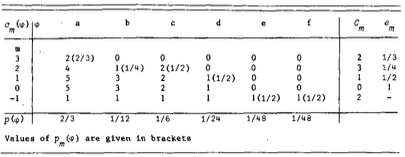
\includegraphics[width=0.75\textwidth]{PPM}
    \caption{Order of PPM \(o_m(\phi)\), Item Probability following context \(p(\phi)\), Total count for items following context of same order \(C_m\), Escape Probability \(e_m\)}
    \label{fig:PPM}
\end{figure}
 
\subsubsection{Markov Chains (All K / 1st order)}{\label{Markov}}
Items from sequences (that belong to a dataset) can be easily imagined as events occurring consecutively after other events. In a 1st order Markov chain, an event solely depends to the previous one. A probability between events can be calculated during the creation of the chain. Hence, through the Markov chain it is shown the possibility of an item appearing after another in the chain. However, an event can't only depend on the previous one. It is possible to have a dependency on the last K events. That formalises the order of the Markov chain. According to the order, an event is solely depends on the previous K events on the path of the chain, hence a conditional probability can be calculated \cite{Pitkow99mininglongest}.
\par \citeauthor{Pitkow99mininglongest} \citeyear{Pitkow99mininglongest} used a hybrid model between a data mining task called \emph{LRS} (\textbf{L}ongest \textbf{R}epeating \textbf{S}ubsequences) and All K (or 1st order) Markov Chains. It is shown how issues regarding Markov chains can be addressed; issues like space complexity and boost of accuracy by discarding infrequently sequences (which are considered as noise).
\subsubsection{Dependency Graphs}
In a dependency graph it is represented dependencies of items towards each other \cite{Padmanabhan:1996:UPP:235160.235164}. When a dependency graph is constructed, an item (let's say B) is associated with another (let's say A), through an arc, if and only if the second (B) occurred  at some point in time after the first item (A). A \emph{look ahead window} size can specify how far a correlation between two items can be. Each arc that correlates two items has a weight which shows the probability of an item occurring after another. Specifically, this weight is not the probability of the item occurring consecutively/immediately after another item but the probability occurring in the specified window. An example of a small dependency graph used for predictions of web pages is shown in Figure \ref{fig:DG}. 

\begin{figure}[h]
    \centering
    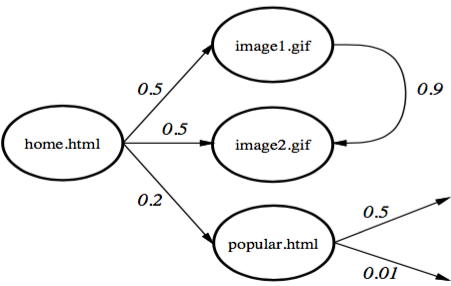
\includegraphics[width=0.4\textwidth]{DG}
    \caption{When a node like home.html is accessed, there is a 50\% chance image1.gif to be access soon afterwards. Same happens for image2.gif. However, even though the specified look ahead window is concrete for the whole graph, each arc may lie in different window vallues (but still equal or less to the look ahead window value)}
    \label{fig:DG}
\end{figure}

\subsubsection{LZ78 \& LZW}
LZ78 and LZW are lossless compression algorithms that can be used for prediction purposes. The most important part about these two algorithms is the dictionary construction algorithms that is used by \citeauthor{Moghaddam_Kabir} \citeyear{Moghaddam_Kabir} in order to create the prediction model \cite{Moghaddam_Kabir}. A prediction tree is constructed by feeding the algorithms with sequences (example with LZ78 shown in Figure \ref{fig:LZ78}). On this example, sequences ABABCBC, ABC and ABCD are inserted. However even though A and C come after B, tree does not depict these items.

\begin{figure}[h]
    \centering
    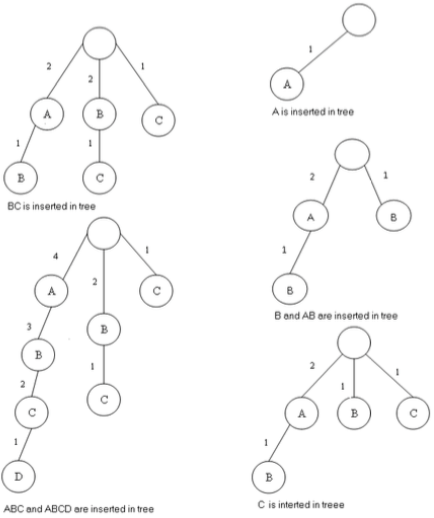
\includegraphics[width=0.50\textwidth]{LZ78}
    \caption{Snapshots of prediction tree that created by LZ78}
    \label{fig:LZ78}
\end{figure}


\subsubsection{Strengths \& Weaknesses}
Lossy approaches lead to models that are more compact and memory efficient in cases when a dataset is more uniform. Let a dataset with quite large repetition of information to be considered. In such case, a lossy approach can represent the dataset without a high memory utilisation in comparison with a lossless approach that has to represent the whole data in a data structure. However, in cases where the datasets are less uniform and relatively big, a lossy model can be very complex and less accurate too.
\par Most of the above approaches assume the Markovian hypothesis where each event solely depends on the previous one. If this hypothesis does not hold, prediction accuracy can severely drop. Also, all these models are built using a part of the information contained in dataset. Therefore, these models do not use all the information contained in given sequences to perform predictions \citep{gueniche_fournier-viger_raman_tseng_2015,gueniche_fournier-viger_tseng_2013}
\subsection{Lossless Approaches}
A lossless sequence prediction approach uses all the dataset's available information to create data structures which are used for predictions. The information that is provided by the dataset is fully reversible to the initial form of the dataset without any loss of information. Therefore, all the available information is used for making predictions.

\subsubsection{Markovian Predictor}
Let the dataset which used for training a predictor to be called \emph{training set} $T$. Given a context, a Markovian predictor has to match the exact context in $T$ and find those sequences that contain that context. For every sequence that contains the exact order of context, the Markovian predictor keeps the item that comes consecutively after the matched context. Finally all these items are gathered in order to get the most frequent one which will be the prediction for the given context. Various Markovian predictors are given in Section\ref{PTonBSFM}.
\subsubsection{Similar Contexts Markovian Predictor}{\label{SCMP}}
Given a context, this predictor looks for sequences in $T$ that simply contain all the items of context in any order and in any position. For any matched sequence in $T$, all the items that come right after the last matched item of the context are considered as candidate predictions. These items are gathered and based on that collections, a prediction is done. Depending on the parameters of the prediction task, the predictor can take into account a number or all the items coming after the matched context and calculate the most frequent item which will be the predicted one. An implementation of such predictor can be seen in Section \ref{CPT}.

\subsection{CPT/+: A Data Structure for Similar Contexts Markovian Predictor} \label{CPT}

CPT and CPT+ (\textbf{C}ompact \textbf{P}rediction \textbf{T}ree) introduced by \citeauthor{gueniche_fournier-viger_tseng_2013} \citeyear{gueniche_fournier-viger_tseng_2013} and later improved by \citeauthor{gueniche_fournier-viger_raman_tseng_2015} \citeyear{gueniche_fournier-viger_raman_tseng_2015}, is currently the only implementation in lossless sequence prediction. It is constituted by a Trie (\emph{Prediction Tree PT}), an Array of bit-vectors (\emph{Inverted Index II}) and an array of pointers to the last items of sequences inserted to the prediction tree (\emph{Look-up Table LT}). As a lossless approach, CPT utilises the whole dataset provided for building its structures. Each sequence from the dataset is inserted to the Prediction Tree and a pointer to the last item of the sequence is added to the Look-up Table. The Inverted Index has the role of finding which sequence contains which alphabet's items by simply executing a bitwise AND operation. Every bit-vector has the same length with the size of the dataset's alphabet while it notes, using 1/0, whether an alphabet item appears in the sequence or not.
\par CPT can retrieve any searching sequence with specific alphabet items by using the inverted index along with a combination of the two other structures. A bitwise AND shows which sequences contain some given alphabet items and then these sequences can be located by using the Look-up Table which points to the end of each corresponding sequence. A detailed way to use this structure for predictions is described in Section \ref{cpt_pred}.

\begin{figure}[h]
    \centering
    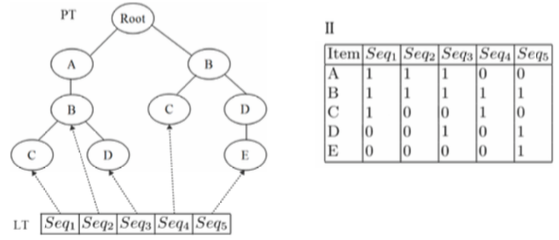
\includegraphics[width=0.75\textwidth]{CPT-structure}
    \caption{A Prediction Tree (PT), Inverted Index (II) and Lookup Table (LT)}
    \label{fig:CPT-structure}
\end{figure}

In Figure \ref{fig:CPT-structure} it is shown an example of CPT during multiple sequence insertions.


\subsubsection{Strengths \& Weaknesses}

As shown in Section \ref{CPT}, CPT utilises all the available sequences in a tree where they are accessible through the II and the LT easily and fast by a bitwise AND for each sequence. Therefore, making predictions can be potentially fast and accurate as described in \citep{gueniche_fournier-viger_tseng_2013} and \citep{gueniche_fournier-viger_raman_tseng_2015}. Locating similar sequences can be a relatively easy task that makes CPT/+ work as a good tool for predictors that exploit such sequences. Moreover, CPT/+ can implement all the prediction tasks described in Section \ref{predtask}, offering a bigger diversity for implementations of several applications. 
\par However, even though with the improvement of CPT, where size of the structures were reduced and speed was  enhanced, some performance issues can be still addressed. Bit-vectors are the main element of II which is used for locating CPT's sequences. When more and more sequences are being added, the bitwise AND operations are becoming slower and slower, leading to performance issues and overall scalability issues since the vectors are becoming much larger. It is common for real life applications to deal with datasets that contain an enormous number of sequences. Therefore, Bit-vectors can be CPT's Achilles' heel regarding its peformance. Also, space usage of II in such cases can be wasteful since with Succinct Data Structures (see Section \ref{SDS}) a better and more memory efficient structure can be proposed.

\subsection{Lossless VS Lossy Approach}{\label{losslessVSlossy}}
Lossless sequence prediction is a relatively new approach and therefore appears to have quite a few challenges that someone that studies it has to cope with. It is clear that due to the fact that a whole dataset is utilised, a lossless approach achieves a higher space utilisation over a lossy approach. This fact leads to two results; firstly, it is somewhat intensive for an algorithm to go through all the data and extract the appropriate information needed for predictions, and secondly, keeping all the relative data \emph{in memory}, through the corresponding data structures, appears to be a considerably hard challenge because the represented structure's space utilisation often reaches an order of magnitude of the initial gathered data. As a result, a lossless sequence prediction approach needs sophisticated tools to search for patterns and sequences in \emph{Big Data} when simultaneously the aforementioned challenges are coped.
\par On contrary, a lossy approach can be less memory hungry by representing the given information of a dataset through models (like dependency graphs). This leads to implementation that sometimes utilises less space and can be potentially faster. However, a lossy approach lacks accuracy especially in hard cases when information in a dataset is not repeating as other parts of informations or a repetition is either generalised or ignored by a model having a partly loss of information that is not reversible. Often such hard cases lead to more complex models that along with Big data is hard to make algorithms that produce predictions with efficiency and performance.

\subsection{Succinct Data Structures}\label{SDS}
This kind of structures are high space efficient data structures (introduced by \citeauthor{Jacobson89} \citeyear{Jacobson89}) that support rapid and efficient operations, (look Appendix \ref{App:rank_select}), like \emph{rank} \& \emph{select} \cite{dillabaugh_2007, Jacobson89}. A data structure in order to be considered \emph{succinct}, it should use space that approaches the information-theoretic lower bound of the space that is required to represent the data. One interesting fact is that in contrast with other compressed representations succinct data structures do not sacrifice performance in order to deliver space efficiency when represent and retrieve back any relative data. 
\subsubsection{Why Succinct Data Structures}
Using \emph{Succinct data structures} can help reducing the space required by a lossless approach and keep most of the data "in memory" (which is stated as a main challenge in Section \ref{losslessVSlossy}). This leaves open room to improve an algorithm's scalability. If we consider that compression methods are mostly based in compression and decompression mechanisms, it is almost clear that much time is spent in compressing and decompressing data. Even though, it would have been achieved a space reduction by using a compression method, the overall performance would not have been any good. Even worse, in a scalable level such an algorithm would take huge amounts of time to complete leaving out an important aspect of the algorithm which is scalability. Also, if we consider prediction tools like backward search on FM-Index (Section \ref{PTonBSFM}) which their complexity to find a search pattern depends only on the times a rank/select were performed, this leads to algorithms which are more scalable with a robust performance time which is in-dependable of the input training set; aspect crucial for an algorithms performance.


\section{Work \& Research}
Part of the work of the Section \ref{PTonBSFM} is motivated through my master's Thesis \cite{ktistakis}. Rest of the work (sections\ref{Prs} \ref{BS_accev} \ref{FurId}) was built on this master's thesis and an accuracy evaluation was done (Section \ref{AccEv}) along with a different evaluation scheme proposals (Section \ref{AccEv}).

\subsection{Evaluation Scheme}{\label{EvSch}}
Evaluating a predictor's accuracy and defining a \emph{scoring mechanism} is a quite difficult and challenging aspect of sequence prediction, as described in Section \ref{plan}. First of all, a prediction task has to be chosen for the predictor that is about to be evaluated. Secondly, the scoring mechanism has to be defined for this chosen prediction task. For example, a calculated prediction by a predictor will have different weight in the final accuracy ratio according to the definition of the scoring mechanism.
\subsubsection{k-fold Validation Environment}
Before defining the evaluation environment, it should be briefly mentioned how the testing environment is set up. The principle that is used is the \emph{k-fold} validation \cite{Kohavi} where in our case the number of folds is 10. For an acquired dataset, it is split in 10 distinct parts (folds) where the 9 folds are used to feed the predictor for training (so these 9 folds are the predictor's training set $T$) and the 10\textsubscript{th} fold is used for testing/evaluating the predictor according to the accuracy evaluation environment. This procedure, training and testing, repeats for 10 times. For every time the k-fold validation is done, a different set of testing and training folds are chosen. The way the sequences from the testing fold are used for obtaining predictions by a predictor is defined by the accuracy evaluation environment. The use of the training folds, clearly depends on the nature of the predictor (lossy/lossless etc. see Section \ref{lit_rev}).
\par\textbf{Implementation Specifications.} Since the existence of the different implementations of the prediction tools, k-fold validation environment had to be adapted and be able to run with all these different implementations. For example, the prediction tool using Backward Search on FM-Index (described in Section  \ref{PTonBSFM}) is implemented in C++ while the prediction tool using CPT+ structure is implemented in Java \cite{gueniche_git}. A solution to unify k-fold validation for different implementations was to set it up in a way that it exports the 10 different sets of folds and then configure other implementations' environment to use these exporting folds. In that way, it is assured that all the predictors are trained and tested under the same circumstances.

\subsection{Accuracy Evaluation Environment}
The accuracy evaluation environment defines how accurate a predictor is according to the executed prediction task.. The predictors' implementation which are mentioned in sections \ref{PTonBSFM} and \ref{cpt_pred} are evaluated under the two scoring mechanisms of prediction tasks which are described below. The predictor is trained using the corresponding training set of sequences (folds) and for a testing set (fold) of sequences $E = \langle Q_1, Q_2, \ldots, Q_{l\prime}\rangle$ every testing sequence $Q_{l\prime}$ is split into two parts. The first part constitutes the context and the remaining second part the suffix. The size of the context and suffix are defined before the evaluation is initialised to run and somehow it is a dependence of the prediction task. Usually, there is the option to spilt a testing sequence into three parts; a prefix, a context and a suffix where the context is used like already described and the prefix is discarded. Why a prefix can be discarded depends on the evaluation scenario that is set up. For example, if the evaluation scenario specifies that the testing sequences are web logs from a user's history when he visited a web page, then it would make sense that the first couple pages (first items of the testing sequence) may be more random user clicks that do not yet define his actual purpose of visit at this very specific web page (when we visit a page, usually, at first we try to familiarise ourself with the content of the page and explore the first couple of pages). For the evaluations that follow during this report, a test sequence is slit in (the aforementioned) three parts. 
\par\textbf{Right next item Scoring}. A context of a query sequence is used for feeding a trained predictor. When a prediction is returned the suffix is used in order to get determined whether this prediction is accurate or not and assign a \emph{score} to this prediction. For this prediction task, the scoring is relatively naive. The suffix size is 1. So, if the prediction happens to be the same item with the suffix's item then the predictor increases its score by 1 (this suffix belongs to the same test sequence like the context for a corresponding prediction). Finally, the score is divided by the overall prediction attempts giving an accuracy rate.
\par\textbf{Item in a future window Scoring}. This scoring mechanism \cite{gueniche_fournier-viger_tseng_2013} depends on the same principle of splitting the testing sequence in three parts. Based on the context, a prediction is returned. The suffix size, also called \emph{consequent length}, is defined before the initialisation of the evaluation procedure. If the prediction item occurs to be any of the items of the suffix/consequent on any position, then the predictor's score is increased by one. Finally, the accuracy rate is the division of the score by the overall prediction attempts.
\par For both scoring mechanisms, a prediction is counted as an attempt even if the predictor does not return an item as a prediction (i.e.\ a context was not matched in a training set by the predictor). In that case, the score is zero and the attempt is counted.

\subsubsection{A proposed evaluation scheme: Multiple Predictions per Sequence}{\label{proposedEv}}
This evaluation scenario combines the Item in a Future Window prediction task and an \emph{LRU} (\emph{L}east \emph{R}ecently \emph{U}sed) mechanism. It is motivated through the fact that a predictor can serve an LRU cache by making the cache taking some advices for which elements to remove from its allocated space. Normally, an LRU cache works like this; If an item is requester by a client that the cache serves, and the item does not appear to be in the cache's memory then the item is retrieved accordingly and placed into the memory. This new item now is placed on top of the cache (we should imagine the cache as a stack) and it is returned to the client that requested that. In a different case that a requested item appears to be in the cache's memory, the item is placed on top of the cache and returned to the client. Every time that the allocated memory which is dedicated to the cache is full, the item that is located on the bottom of the cache is removed and it does not longer belong to the cache's memory.
\par On this evaluation method, the prediction task serves a cache memory that uses the LRU mechanism. The cache mechanism decides which element to insert into the memory based on suggestions made by a predictor. The cache could have the chance not to every time listen to the predictor's suggestions, since fetching elements in the cache that are not being used, increases the cache's resources. So, whether an element will be put in the cache or not, could be decided according to a threshold parameter which is based on a confidence of a prediction (Section \ref{Prs}). A predictor tracks the client that makes the requests to the cache and then suggests to the cache items that soon will be requested be the client. Hence, when the client requests an item, it is very possible to already be in the memory. This makes the cache more efficient since, for example, it will not be spent time on retrieving the requested item from a database storage. However, if the predictor's suggestions are not accurate and the items that the cache puts in are not requested by a client then the spent resources of the cache are increased without any actual benefit to the client's experience (i.e.\ faster cache response). Thus, a cost/benefit mechanism is proposed in Table \ref{table:cache_score}. According to this table the scoring is defined like that; whether the prediction exists in cache or not the cost is increased accordingly since if the predicted item is not in the memory, it has to get retrieved and put in. The same happens for the client's request item. However, if a requested item is already in the cache memory, the benefit is increased since a prediction becomes useful.
\par\textbf{Multiple Predictions per Sequence}. This title comes from the fact that instead of using a test sequence for one prediction (derive the context/suffix and produce a prediction according to the context), we can use a test sequence for producing multiple predictions. Having fixed the size of the context (as $contextSize$), the evaluation is started from the test sequence's start and the first $contextSize$ items are given as a context to the predictor. The result of the predictor is put in the cache memory (like described already). Then the $contextSize+1$ item of the test sequence is requested from the cache. The evaluation environment will observe whether the requested item was already in the memory or not and assign the relevant score. The procedure will continue with the same test sequence but now beginning from the second item of the sequence to the ($contextSize+1$)-th one while the $contextSize+2$ will be requested from the cache. This will continue until the point the generated context reaches the end of the test sequence (actually one item before the end, since the last item is needed as a request to the cache).
\begin{table}[h!]
\centering
\begin{tabular}{ |c|c|c| } 
 \hline
  & \textbf{Cost} & \textbf{Benefit} \\ 
 \textbf{prediction \(\in\) cache \(\wedge\) client's request item \(\in\) cache} & 0 & 1 \\ 
 \textbf{prediction \(\notin\) cache \(\wedge\) client's request item \(\in\) cache} & 1 & 1 \\
 \textbf{prediction \(\in\) cache \(\wedge\) client's request item \(\notin\) cache} & 1 & 0 \\
 \textbf{prediction \(\notin\) cache \(\wedge\) client's request item \(\notin\) cache} & 2 & 0 \\ 
 \hline
\end{tabular}
\caption{Score Definition for a Cache that uses prediction advises}
\label{table:cache_score}
\end{table}


\subsection{Prediction tool using Backward Search on FM-Index}{\label{PTonBSFM}}
Backward Search on FM-Index, description on appendix \ref{App:bs_fm} can be a powerful sophisticated tool which can be used by a Markovian Predictor and not only. With backward search and the utilisation of rank queries (appendix \ref{App:rank_select}) we can get the location of all the occurrences of a search pattern in a sequence of items. Having the context and the training set $T$, backward search on $T$ will return a \emph{range} where all occurrences of context lie in $T$. That means that it is possible to find every item coming consecutively after each occurrence, giving a tool for implementing a Markovian predictor. One technical detail on this fact is that the returned range from a backward search gives occurrences of what comes consecutively \emph{before} the searched context \cite{ktistakis}. However, if both $T$ and context are reversed, backward search gives the occurrences of items which come \emph{consecutively after}. What is worth noting with this prediction tool is that offers a way of representing $T$ utilising low memory space (with the use of succinct data structures) and a way to get a robust execution time for performing predictions without depending on the size of $T$.
 
\subsubsection{Predictors}{\label{Prs}}
The range obtained by the backward search can be used in order to get the most frequent item (located among the range items) coming consecutively after the context. A naive way of doing that is by just going through all items of the range and calculating the frequencies \cite{ktistakis}. However, if the range is quite long this could take time, making the predictor unusable in cases where a context matched in $T$ quite a few times. An alternative way was investigated during my Master Thesis where the most frequent item could get calculated by performing rank operation calls, in the obtained range, for every alphabet item of $T$. This method provides the frequencies for all alphabet in a range and can easily give the most frequent one which will be the final prediction. If the range is relatively small and the alphabet size quite big then this method is not efficient at all. So, a threshold was proposed \cite{ktistakis} where the aforementioned methods could be used in different situations accordingly.

\par One of the problems of the described prediction approach (studied during my Master Thesis) is that the exact context is searched in $T$, making the number of times context matched in $T$ low (especially when context is somewhat long). Which means that the \emph{coverage} of a prediction is low. Coverage is defined as the ratio \(\vert no\_matches \vert /\vert sequences \ in\ T \vert\). Some modifications to the previous described algorithm could increase the coverage and it is described below (which were studied, implemented and evaluated during the 1\textsuperscript{st} year of my PhD research).

\par \textbf{Recursive Divider}. A prediction algorithm idea which was firstly introduced by \citeauthor{gueniche_fournier-viger_tseng_2013} \citeyear{gueniche_fournier-viger_tseng_2013} and applied on CPT/+ (see Section \ref{cpt_pred}). The main idea is to recursively derive subsequences from a given context and try to perform prediction using all these derived subsequences. This approach work for $d = 1,2,\ldots maxLevel$, where $maxLevel$ is the maximum length ( and less or equal to context length) of derived subsequences to explore. Each subsequence's prediction has a different \emph{weight} ratio according to the $d$ level value of the subsequence. The recursion stops when all levels of subsequences are explored or a prediction is achieved during the exploration of a level.

\par \textbf{Prediction based on Confidence}. There is a case where during a prediction, a candidate for prediction item is the same possible as another(s). In that case, the overall \emph{Confidence} of the item is calculated. The item among the candidates that has the highest Confidence is then the one that is predicted. Confidence of an item is defined as the ratio \(item\_frequency/\#sequences\) in $T$.

\par \textbf{Unseen/less confident Items Removal}. Sometimes, it was observed that accuracy was boosted when less confident items or even unseen items (considered as noise, but it is not the case in our evaluation environment) are removed from the context before this context is given to the predictor. A pre-defined parameter can limit the context to contain items that have a specific confidence ratio. Then, these items are removed and a prediction is initiated. 

\par An accuracy comparison made between the simple Markovian Predictor (using backward search tool without any optimisations) and the optimisations implemented (Recursive Divider, Prediction based on Confidence and Unseen/less confident Items Removal) is shown in Section \ref{BS_accev}.

\subsubsection{Accuracy Evaluation}{\label{BS_accev}}
An accuracy evaluation of the predictor (and its later proposed optimisations, Section \ref{Prs}) was not part of the Master Thesis, however it is crucial to observe the accuracy behaviour of the predictor with the backward search tool. In Figures \ref{fig:bs_pred_Ev1} and \ref{fig:bs_pred_Ev2}, it is depicted the ratio of answers (coverage) and the ratio of success (predictions which are marked as accurate). The datasets used for this accuracy evaluation (and for the next evaluations) are part of the spmf data mining library \citep{spmf} which mainly offer sequence collections of click stream data from various websites.
\par \textbf{Successful Prediction}, for this evaluation purpose, is defined as an accurate prediction only if the predicted result happens to be the 1\textsuperscript{st} item of the test sequence's suffix. The number of the successful predictions divided by the number of overall prediction questions, defines the success rate.
\par As observed in Figures \ref{fig:bs_pred_Ev1}, \ref{fig:bs_pred_Ev2} both accuracy and as a result and success rate are boosted, especially in cases where the context is increasing. The main reason of that is that recursive divider explores more possible contexts in cases when the initial context was hard to matched in $T$.



\begin{figure}[h]
    \centering
    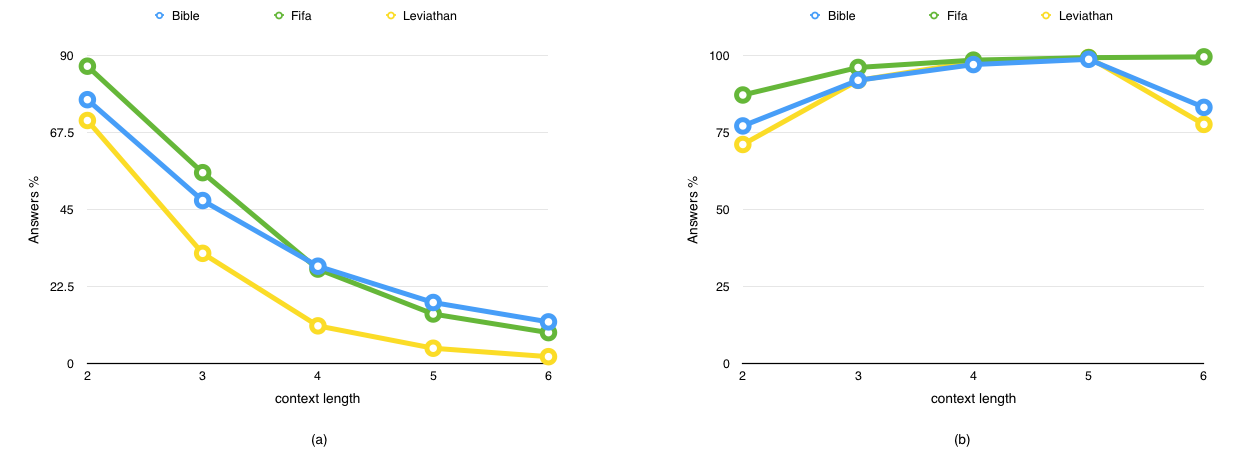
\includegraphics[width=1\textwidth]{rec_div_answers}
    \caption{Ratio of answers: Recursive Divider is off (a) and on (b)}
    \label{fig:bs_pred_Ev1}
\end{figure}

\begin{figure}[h]
    \centering
    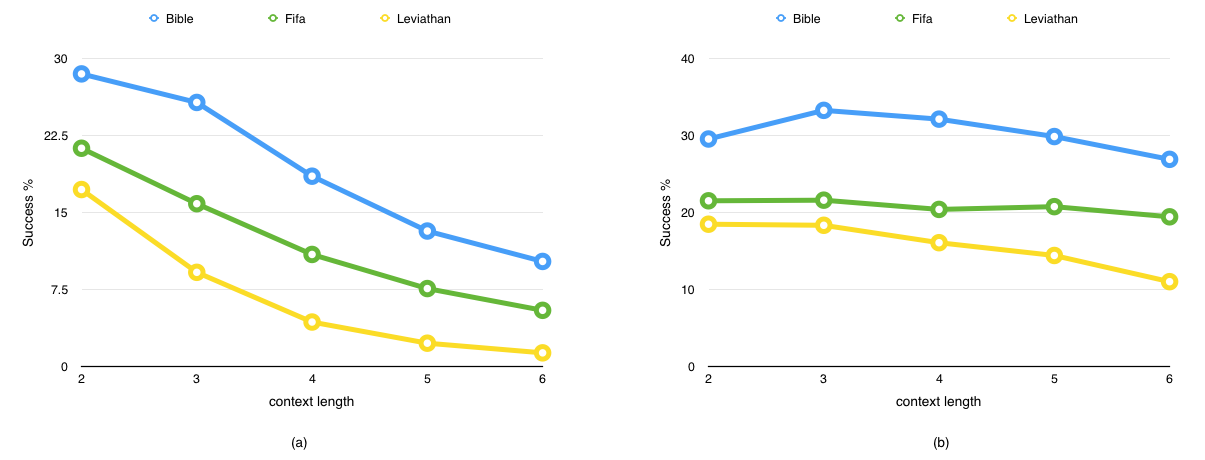
\includegraphics[width=1\textwidth]{rec_div_succ}
    \caption{Ratio of success: Recursive Divider is off (a) and on (b)}
    \label{fig:bs_pred_Ev2}
\end{figure}


\subsubsection{Further ideas for predictors}{\label{FurId}}
As stated in Section \ref{plan}, one of the main research targets is to find new predictors and then identify appropriate (succinct) data structures in order to achieve both accuracy and performance (speed and memory efficiency).
\par A predictor idea is based on the problem of \emph{document listing}\footnote{The idea in this section and in the corresponding appendix section obtained from a lecture of Simon Puglisi available \href{https://sites.google.com/site/ku2015topicsindatamining/home/lecture2.2.pdf?attredirects=0&d=1}{here}}. The problem lies on the next fact; having a collection of strings (which we can call documents), the problem is to find all the documents ( or strings) that contain a query pattern. Later, it will be shown that CPT/+'s predictor is based on the same principle of document listing. When a predictor accepts a context from a test sequence, an idea is to find all the sequences from $T$ that contain this very specific context. If the idea gets more specific some details vary but from a general view the main principle of document listing is the same. Until now, backward search tool used in order to implement an efficient Markovian Predictor. On the other hand backward search can be used in order to solve the problem of document listing and implement a new predictor. Such a solution is shown in appendix \ref{App:bs_doclist}. The advantages of using backward search for document listing is that a memory and speed efficiency is achieved since the time needed to list the documents containing a specific patter is almost the same with the time needed to perform a backward search for the same pattern. 
\par Since all the sequences that contain a specific context (called matched sequences) can be derived from $T$, it is then easy from the matched sequence to separate the part that contains the context and the part that is consecutive after that context. The part consecutively after the context (see Section \ref{pre_def}) can be used for calculating any predictions with different ways.

\subsection{Prediction tool using CPT/+}{\label{cpt_pred}}
CPT's structure has already seen in Section \ref{CPT} where it was showed how to insert sequences from a training part of a dataset. CPT structure, though, can be used in order to implement a Similar Contexts Markoviain Predictor (Section \ref{SCMP}). Having a context from a test sequence, CPT can locate the items of the context that are contained in sequences stored in PT. The located sequences, otherwise matched sequences, contain the items of the context in any order and in any position. For example, let us assume a prediction tree like the one in Figure \ref{fig:cpt_predict} and a context to search $\langle A,B\rangle$. Firstly, the items $A$ and $B$ of the context are spotted in the inverted index. For each located item in the II, it is found which sequence contains every corresponding item (in this case $A$ and $B$). Then, it is performed a bitwise AND operation on the appropriate bit-vectors of $A$ and $B$ in order to locate which sequences simultaneously contain both $A$ and $B$. These sequences are $S_1$, $S_2$ and $S_3$. Next, all (or a part of; this part can be defined prior to predictor's execution with a parameter called \emph{Consequent Size}) the items of the matched sequences that occur after the last matched item of the context are inserted into a \emph{Count Table} (\emph{CT}). CT is a table that counts the occurrences of the inserted items and can easily show the most frequent(s) one(s). In this case, $\langle \$, C, D, C \rangle$ are inserted into CT where \$ denotes that for a matched sequence (like the $\langle A, B \rangle$) there wasn't any item occuring consecutively after. 

\begin{figure}[h]
    \centering
    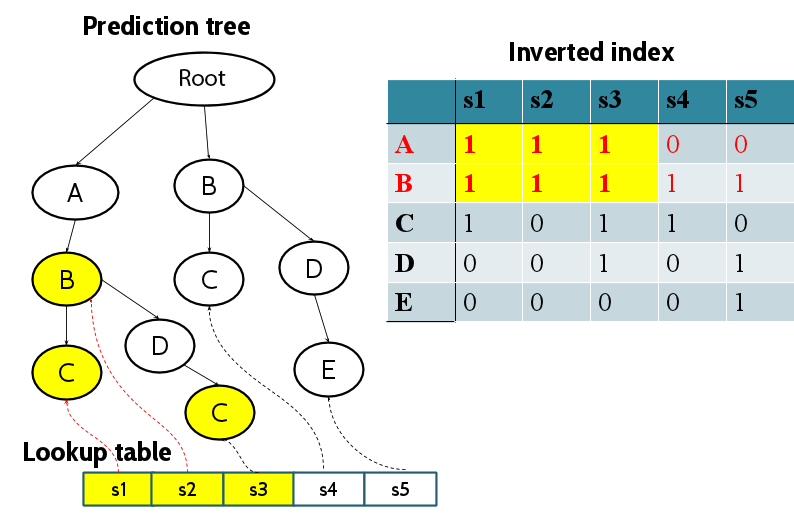
\includegraphics[width=0.75\textwidth]{cpt_predict}
    \caption{CPT structure used for predictions}
    \label{fig:cpt_predict}
\end{figure}

\subsubsection{Accuracy Evaluation}{\label{AccEv}}
In Figure \ref{fig:cpt_predict_accuracy}, it is shown the percentage of accuracy of CPT and CPT+ for a fixed size context of size items and a variable consequent size between one to three items. This means that if a prediction was appearing in the next three items of the test sequence after the matched context, then the prediction was being considered as accurate. It is interesting to observer that the accuracy is being boosted as the consequent length is increased. In applications where this kind of prediction task (Item in a future window) is useful, the CPT/+'s accuracy rate can be considered important since the predicted items are eventually items that indeed occur. The CPT and later CPT+ make use of the Recursive Divider which is described already; with CPT+ having a more generalised implementation of this algorithm.
\begin{figure}[h]
    \centering
    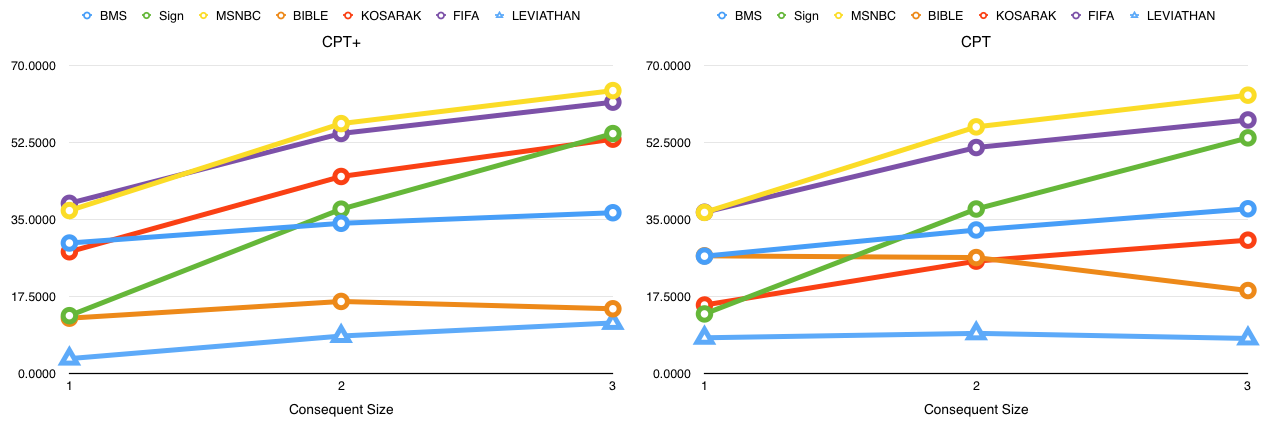
\includegraphics[width=1\textwidth]{cpt_predict_accuracy}
    \caption{CPT and CPT+ accuracy rate for a context length 6 and a varied consequent size}
    \label{fig:cpt_predict_accuracy}
\end{figure}

\subsubsection{Improving CPT/+ Performance}{\label{cpt_improv}}
One of the main CPT's structural elements is its Inverted Index (II) which is constituted by an array of bit-vectors. This specific implementation of the II (which serves one aspect the document listing problem \cite{tabei_tsuda_2011}, appendix \ref{App:bs_doclist}) can affect overall performance in cases where the input dataset grows enough. Such performance issues can be its time needed to perform predictions (and hence much less scalable) and the overall memory consumption. Below is presented some alternative ways of implementing the II where the memory consumptions are being studied among different (succinct) structures.

\par\textbf{RRR Vector as a space improvement}. Instead of using an array of simple bit-vectors, it would be much more space efficient to use an array of RRR-Vectors \cite{Raman}. This kind of vectors are compressed bit-vectors that use rank and select operation calls (appendix \ref{App:rank_select}) in order to represent and retrieve their binary data. The structure of II does not significantly change since it uses a more compressed version of a bit-vector. 

\par\textbf{Wavelet Tree as an Inverted Index}. Wavelet Trees (described in appendix \ref{App:WT}) as a bit-vector hierarchy can be very space efficient for offering the functionalities of the II. The use of a wavelet tree as a solution to the document listing problem proposed by \citeauthor{tabei_tsuda_2011} \citeyear{tabei_tsuda_2011}. A comparison with other proposed structures (which are targeted for document listing) is shown on Figure \ref{fig:IIs_cmp}.

\par\textbf{Multibit Tree as an Inverted Index}. A different succinct representation proposed by \citeauthor{tabei_2012} \citeyear{tabei_2012} where similarity search (document listing) can be achieved by using a Multibit Tree.

Looking at Figure \ref{fig:IIs_cmp}, wavelet trees achieve the best possible compression in every case while the space difference with pure bit-vectors is relatively big. In addition, if it is considered for the whole CPT+ structure implementation, the II takes most of the required space (see Figure \ref{fig:CPT_trie_space}) then it is important to improve space efficiency of the way similar sequences are retrieved through an II.


\begin{figure}[h]
    \centering
    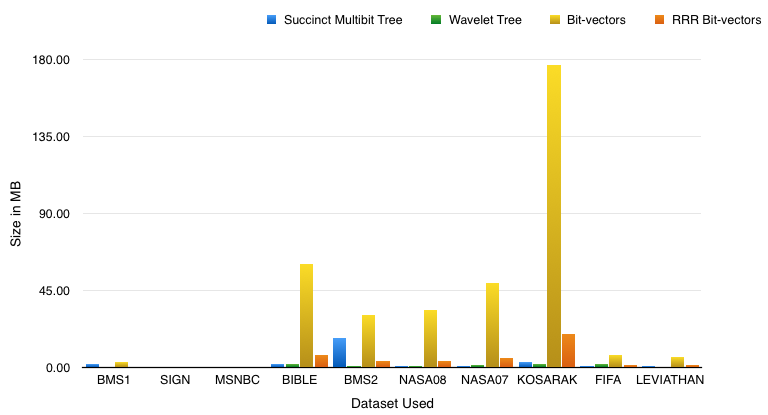
\includegraphics[width=0.75\textwidth]{IIs_cmp}
    \caption{Comparison of succinct data structures with Bit-vector as IIs}
    \label{fig:IIs_cmp}
\end{figure}


\begin{figure}[h]
    \centering
    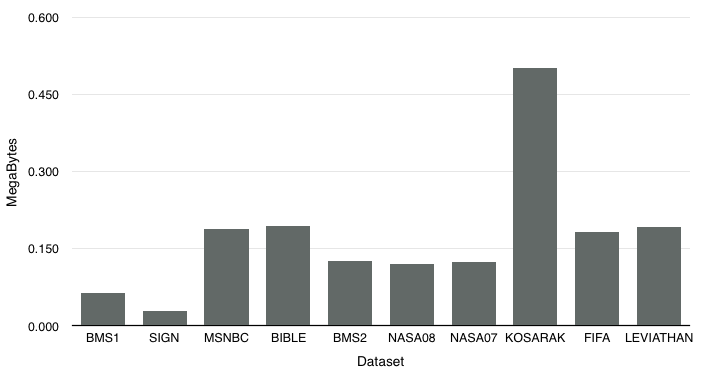
\includegraphics[width=0.75\textwidth]{CPT_trie_space}
    \caption{CPT+ Trie estimated space usage per dataset}
    \label{fig:CPT_trie_space}
\end{figure}



\subsection{Predictors Evaluation}
In this section different predictors are being evaluated according to their accuracy rate. In figures \ref{fig:various_predictors_acc_1} and \ref{fig:various_predictors_acc_2} it is shown their accuracy rate for the ``right next Item" prediction task according to a variable context length. The predictors \cite{gueniche_git} that are compared are the Markovian predictor using backward search on FM-Index (Section \ref{Prs}), the Dependency Graph predictor, All-k-Order Markov Chains predictor, First order Markov Chains (PPM) predictor, LZ78 predictor and the Markov Trees (TDAG) predictor. CPT+ seems to be the most accurate in three out of four datasets while on Bible dataset lies among the middle (and sometimes backward search predictor is closely accurate). Backward search prediction tool lies, in general, around the middle for most datasets while it has better accuracy in only one case (MSNBC dataset).
\par In figures \ref{fig:scatter1} and \ref{fig:scatter2} it is shown some cost/benefit scatter plots which illustrate a main idea of how the benefit is distributed opposite the cost of the evaluation scenario described in Section \ref{proposedEv}. What is interesting to observe is that the prediction tool on backward search (noted as \emph{BWT} on the scatter plot) achieves much better benefit over cost ratio in comparison to other predictors. There is a case that a predictor may achieve a benefit high enough but the cost is also increased which means that some of its predictions are being retrieved into the cache without any future use by a request. Also, it was considered as interesting to observe the behaviour of a cache without taking any advises from a predictor (noted as \emph{No Predictor} on the scatter plot). That means that the evaluation was run as described already but the step for inserting the predicted items into the cache was being omitted. So, only the items that was being requested was eventually inserted into the caches memory (if they were not in). With this tactic, we can observe how much some predictors help according to a current benefit/cost ratio.


\begin{figure}[h]
    \centering
    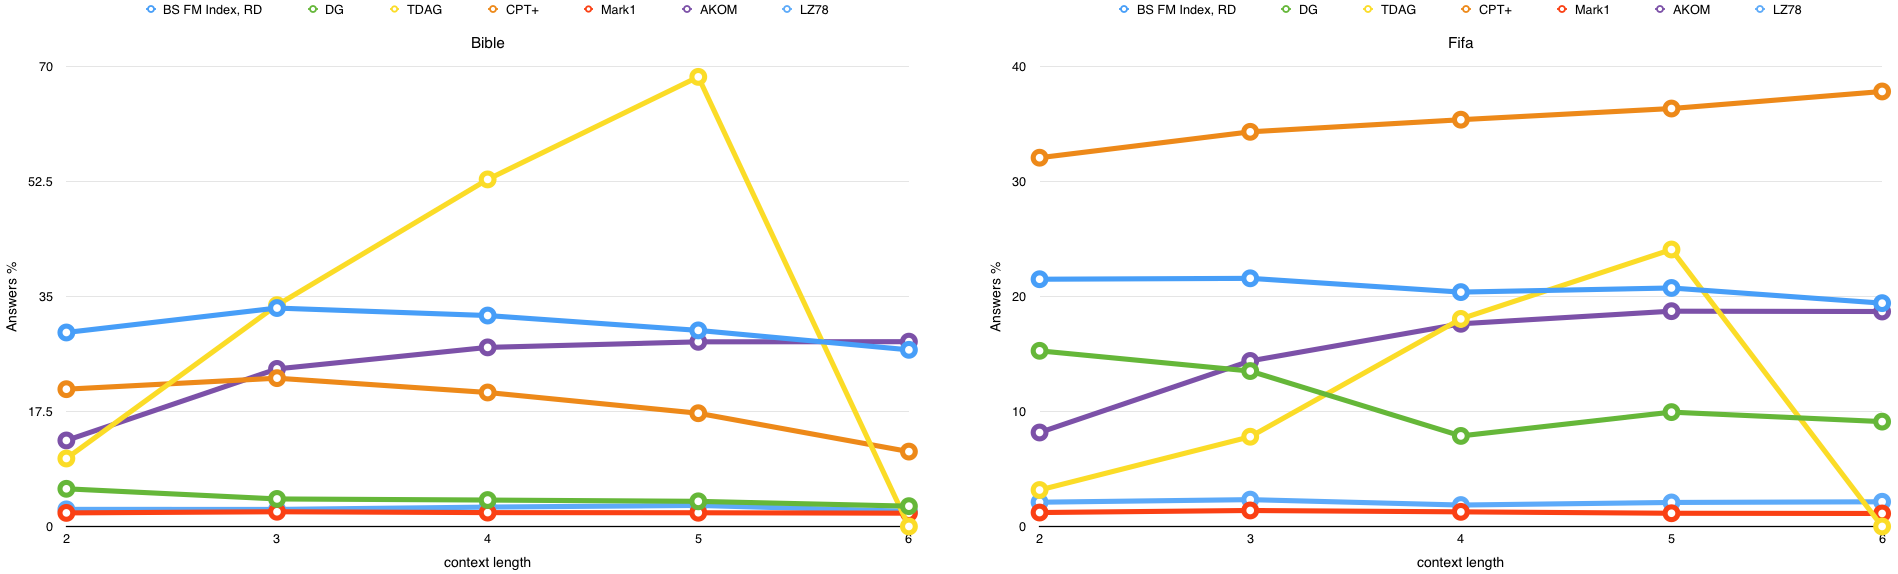
\includegraphics[width=1\textwidth]{various_predictors_acc_1}
    \caption{Various Predictors' Accuracy on Bible and Fifa Datasets}
    \label{fig:various_predictors_acc_1}
\end{figure}

\begin{figure}[h]
    \centering
    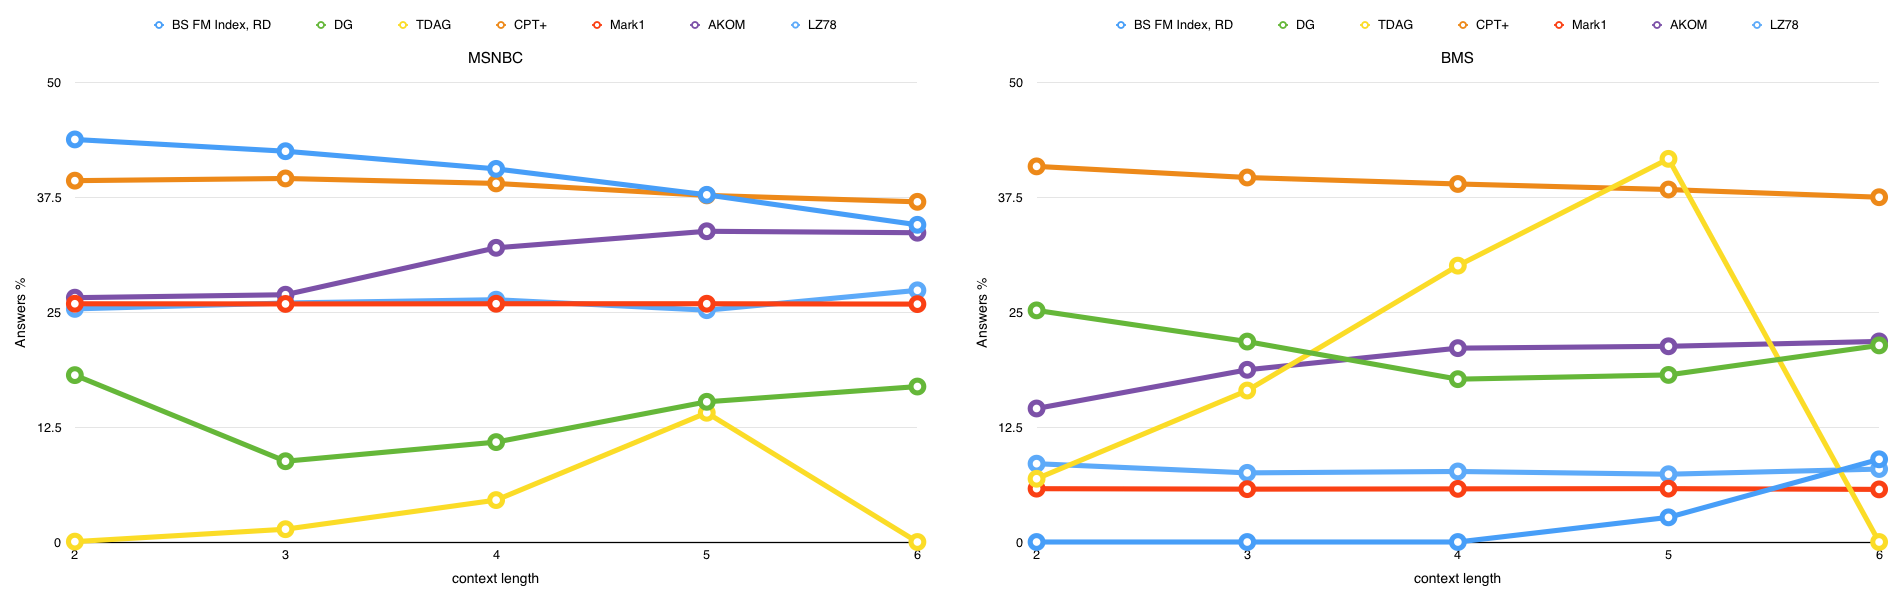
\includegraphics[width=1\textwidth]{various_predictors_acc_2}
    \caption{Various Predictors' Accuracy on MSNBC and BMS Datasets}
    \label{fig:various_predictors_acc_2}
\end{figure}

\begin{figure}
\centering
\begin{subfigure}{.5\textwidth}
  \centering
  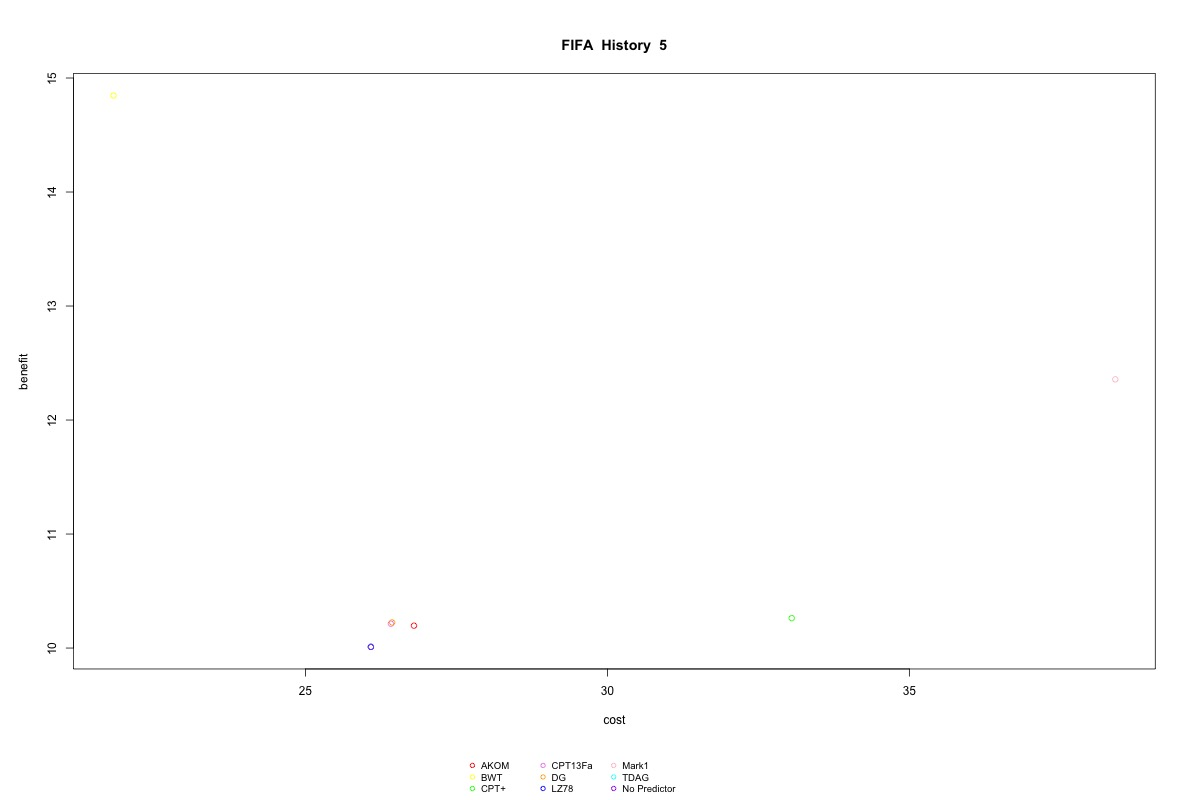
\includegraphics[width=1\linewidth]{fifa_scatter}
  \caption{Fifa Dataset}
  \label{fig:scatter1_sub1}
\end{subfigure}%
\begin{subfigure}{.5\textwidth}
  \centering
  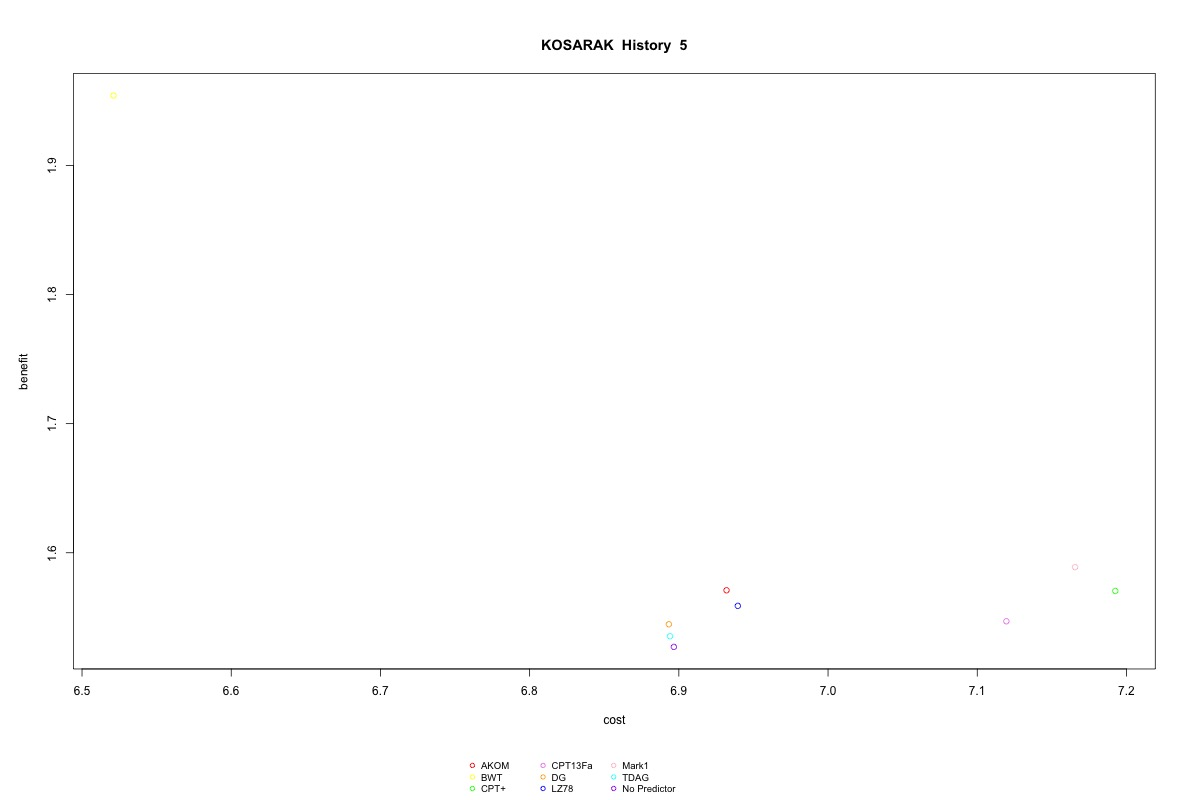
\includegraphics[width=1\linewidth]{kosarak_scatter}
  \caption{Kosarak Dataset}
  \label{fig:scatter1_sub2}
\end{subfigure}
\caption{Scatter Plots for cost/benefit of a Cache that uses advises from various predictors}
\label{fig:scatter1}
\end{figure}

\begin{figure}
\centering
\begin{subfigure}{.5\textwidth}
  \centering
  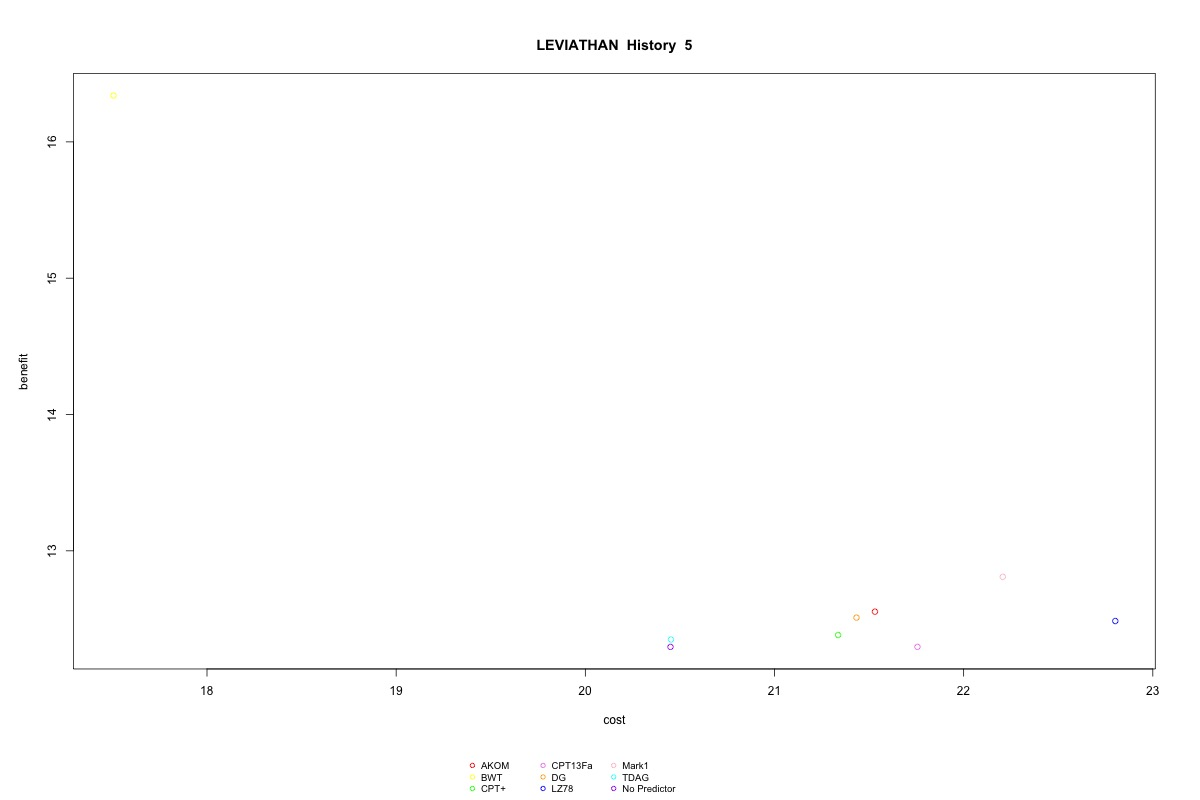
\includegraphics[width=1\linewidth]{leviathan_scatter}
  \caption{Leviathan Dataset}
  \label{fig:scatter2_sub1}
\end{subfigure}%
\begin{subfigure}{.5\textwidth}
  \centering
  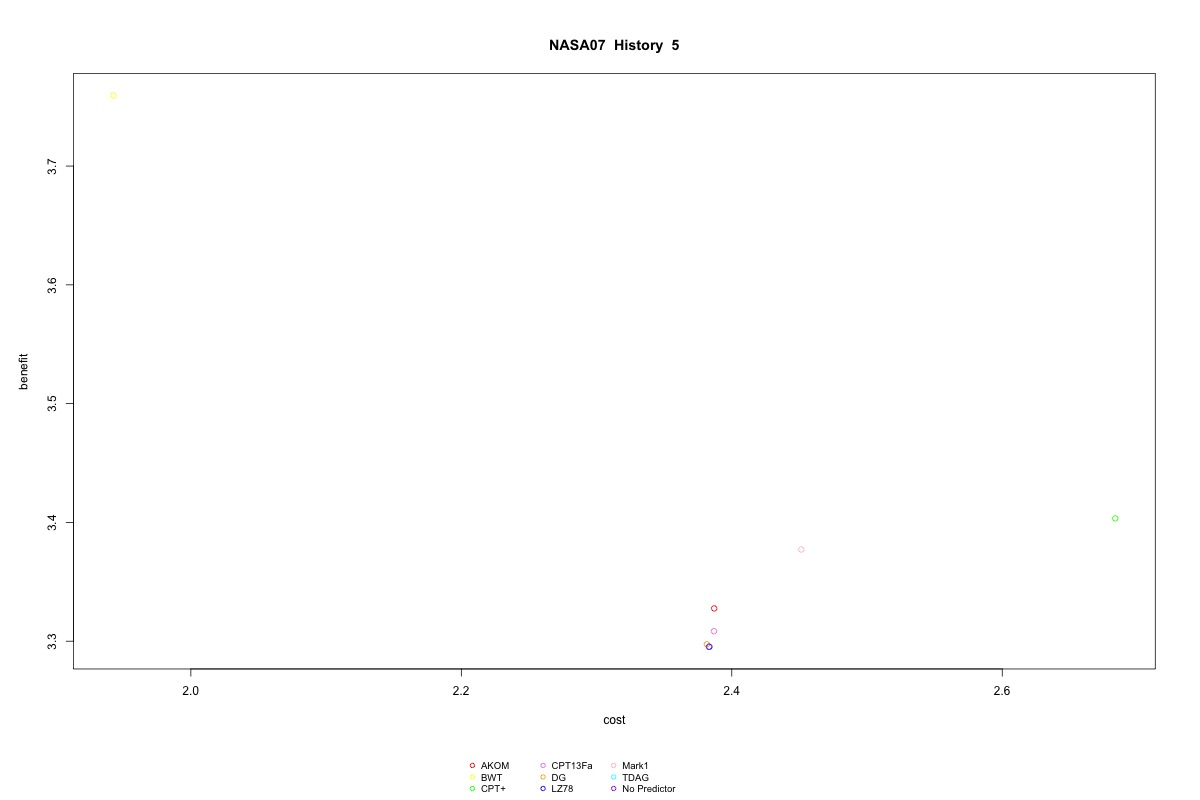
\includegraphics[width=1\linewidth]{nasa_scatter}
  \caption{Nasa Dataset}
  \label{fig:scatter2_sub2}
\end{subfigure}
\caption{Scatter Plots for cost/benefit of a Cache that uses advises from various predictors}
\label{fig:scatter2}
\end{figure}

\subsection{Further research}
\subsubsection{CPT/+ Scalability test}
A CPT/+ scalability test will expose potential issues for its time performance. As CPT/+'s input dataset becomes larger and larger, if the time needed for making a prediction for a given context gets more and more then this makes the whole structure less scalable. Hence, a next scalability test with the adoption of the proposed improvements (Section \ref{cpt_improv}) could show how CPT/+ can be more scalable. Some of the CPT's scalability tests have been done but the results have not yet been studied deeply. For this evaluation, it is important to use datasets that are customised to the needs of the experiments. Hence, a \emph{Synthetic Data Generator} is used in order to generate datasets with fixed attributes. For example, we may need a set of datasets that have a fixed length for every sequence, a fixed alphabet size and a variable number of sequences. That way, it can be observed the behaviour of an experiment over one variable attribute of a dataset and expose potential scalability issues. \par CPT's execution time for performing predictions seems to mainly depend on the size of the input dataset. Due to the fact that its II gets bigger and bigger for more and more sequences, it is common logic that the bit-vectors (the II consists of) will become slower and slower for performing operations. An experiment like the one described above, exposes such vulnerabilities.
\subsubsection{Accurate Predictors Investigation}
Lossless sequence prediction can be considered as a new approach. Several predictors based on this approach can be investigated and compare their accuracy to any existent approach. With the introduction of succinct data structures the end result could be more efficient and robust prediction algorithms regarding their time performance and their memory consumption. With the current implementation of CPT/+ it would be easy to explore many different lossless predictors since the CPT's structure is quite adaptable and flexible on retrieve and matching sequences in the training set with several ways. Hence, a first idea whether a predictor is accurate or not can be obtained easily and then it can be tried to adopt the appropriate data structures for coming through any aforementioned challenges. 
\subsubsection{Scoring mechanisms}
It is already mentioned that a evaluating a predictor can be one of the main challenges of this Thesis. Any proposed evaluation has to be solid and fair among different predictors and be able to distinguish cases with different accuracy weights. For example, if a continuously repeated event is predicted, it should be awarded less over an event that rarely occurs but it is predicted correctly. Such evaluation schemes could offer a better scale for comparisons among predictors of different nature. It would be important to introduce and explore new terms. Such term could be \emph{Shannon's entropy}. Lastly, it would be considered a more broader type of measure for evaluations like the one proposed in Section \ref{proposedEv}. Such measure can be a \emph{Binary Classification Performances} measure \cite{2_kohl_2012} which will give a better understanding when evaluating results with different outcomes.

\newpage

\section{First Year Training}

During my 1\textsuperscript{st} year of my PhD studies, I had followed or planned to complete soon the following trainings:

\begin{itemize}
   \item  General Short Courses
   \begin{itemize}
     \item  Preparing to Teach in Higher Education (Small Group Teaching, Assessment and Feedback, Supporting Student Learning); Certification acquired
   \end{itemize}
   \begin{itemize}
     \item Introduction to LaTeX. Simple ``do it yourself" course, available online at department’s web page; Completed
   \end{itemize}
   \item Departmental Short Courses
   \begin{itemize}
     \item Machine Learning
   \end{itemize}  
   \begin{itemize}
     \item Succinct Data Structures
   \end{itemize}
   \item Departmental Courses
   \begin{itemize}
     \item Compression Methods for Multimedia, CO7096 by Prof. Rajeev Raman; Attended during 2\textsubscript{nd} semester in 2015
   \end{itemize}
   \item External Trainings
   \begin{itemize}
     \item WCTA, Spire2015; Attended in September 2015
   \end{itemize}
   \begin{itemize}
     \item Departmental Seminars 2015
   \end{itemize}
   \begin{itemize}
     \item Graduate School Induction
   \end{itemize}
   \begin{itemize}
     \item International Winter School on Big Data (Bilbao, Spain); (Registered) It will be attended between 7\textsubscript{th} to 12\textsubscript{th} February 2016
   \end{itemize}
 \end{itemize}
 
  \newpage
 
 \section{Plan of the Research Phase}{\label{plan}}
If we want to distinguish the thesis in concrete parts, this can be done by defining three main plans which are:
\begin{itemize}
   \item  Support sequence prediction algorithms with scalable, robust and predictable performance's data structures
   \item Investigate or develop more accurate predictors for sequence prediction applications
   \item Explore appropriate ways to evaluate predictors
 \end{itemize}
\par\textbf{Challenges.} The challenges for the aforementioned plan can be various. First of all, evaluating sequence prediction algorithms is not a very clear procedure with clear steps. There has to be a careful consideration on how to evaluate such algorithms and introduce proper ways which are able to be motivated through real applications. A simple accuracy rate that is the ratio of correct answers over the overall number of answers does not always give the true picture whether the calculated rate is indeed useful to real life applications. Thus, some preliminary work has been done with proposing a different evaluation scheme in Section \ref{proposedEv}. Moreover, having adopted structures for an algorithm that makes the algorithm simultaneously space and time efficient is not always viable and can be challenging. For such cases, we may have to explore more efficient or even different kind of data structures that are not implemented\footnote{For the work described during the previous sections, a succinct data structure library was used which offers an expanding collection of different implementations of those kind of structures \cite{gog_2015}}.

\par A short-term plan for the 2\textsuperscript{nd} year is depicted on Figure \ref{fig:timeplan}. A long-term plan for the 3\textsuperscript{rd} year of the research will be to explore in a further detail evaluation methods for the predictors investigated during the 2\textsuperscript{nd} year. Since this exploration is challenging and a predictor's evaluation is not a clear task, summarising results and reverting back for investigating different ways may be necessary. Investigating predictors, finding appropriate structures for predictors, exploring evaluation methods are tasks that demand a fair amount of work and sometimes is not a straight forward procedure. During the 2\textsuperscript{nd} half of the 2\textsuperscript{nd} year, it will have been provided a preliminary amount of work on coding some predictors with appropriate structures along with some evaluation methods. However the 3\textsuperscript{rd} year will mostly concentrated on those challenging tasks according to 2\textsuperscript{nd} year's feedback which will be important for setting the 3\textsuperscript{rd} year's plan.


\begin{figure}[h]
    \centering
    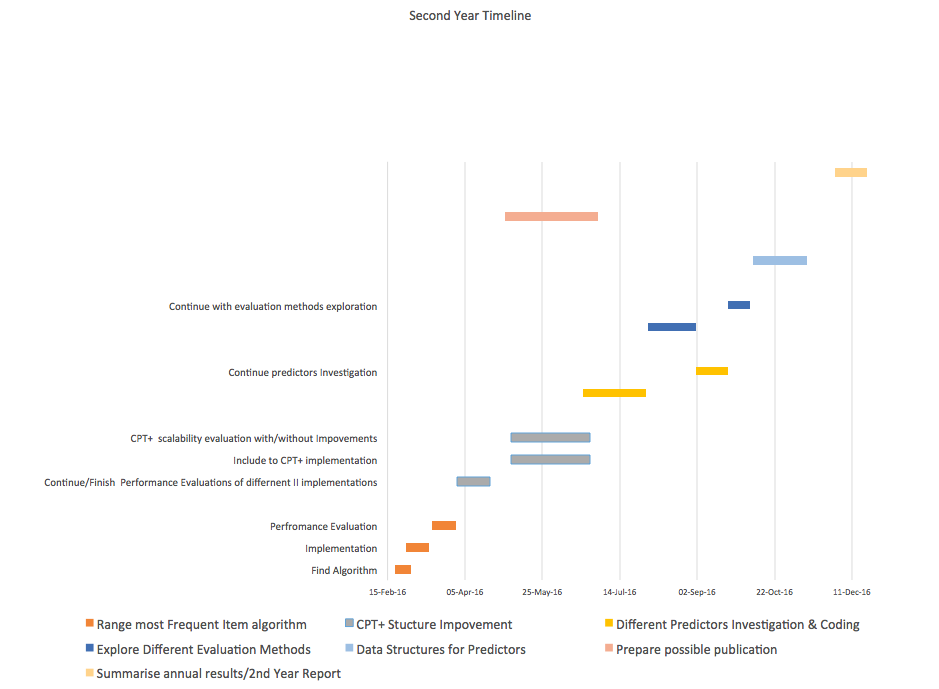
\includegraphics[width=0.7\textwidth]{timeline_plan}
    \caption{Tasks that will take place during the 2\textsuperscript{nd} year of the research}
    \label{fig:timeplan}
\end{figure}


 \newpage